\documentclass[a4paper,10pt]{article}
\usepackage[margin=2.5cm]{geometry}
\usepackage[utf8]{inputenc}
\usepackage[colorlinks=true,urlcolor=blue]{hyperref}
\usepackage{amsmath}
\usepackage{graphicx}
\usepackage{float}
\usepackage{caption}
\usepackage{subcaption}
\usepackage{xcolor}

%\usepackage{listings} %Alternative to minted
\usepackage{minted}

% Template instructions are kept in red; open points are in orange. Remove both before submitting.
\newcommand{\instructions}[1]{\textcolor{red}{#1}}
\newcommand{\TODO}[1]{\textcolor{orange}{\textbf{[TODO: #1]}}}


\setlength{\parindent}{0em}
\setlength{\parskip}{1em}

\title{\textbf{1RT730 Project Report}
	\\ Anime Watching Companion: a tool-planning LLM agent in production \TODO{confirm title}}
\author{Tommi Bimbato, Muhammad Aufa Helfiandri, German David \TODO{full names}}
\date{\today}

\begin{document}

\maketitle

 \section{Introduction}
 \instructions{In this section, provide a brief overview of the LLM application you developed. Explain the motivation behind creating this application (e.g., automation, accessibility, research, productivity). Clearly state the specific problem or challenge that your application aims to address, and explain its significance in a broader societal context. Briefly summarize the main contributions or goals of your work.}

Anime catalogues are large: the AniList snapshot used in this project covers 20,428 titles~\cite{anilist_kaggle}. Viewers who want to choose what to watch next, or to recall who a character is, typically browse several websites or ask a general-purpose chatbot. Such a chatbot answers from its parametric knowledge and may produce fluent but unsupported content, such as invented titles or confused characters~\cite{ji2023hallucination}. Retrieval-augmented generation (RAG) mitigates this problem by conditioning the answer on retrieved evidence~\cite{lewis2020rag}.

We present the \emph{Anime Watching Companion}, a conversational assistant that answers questions about anime and characters and recommends titles, grounding each answer in a structured snapshot of the AniList catalogue. Instead of retrieving text passages only, a planner LLM selects catalogue tools (exact SQL look-ups, attribute filters and semantic search), and a second LLM writes the answer from the retrieved evidence alone. The second aim of the project is deployment: the assistant runs as a web application on Amazon Web Services (AWS), with passwordless sign-in restricted to Uppsala University e-mail addresses, infrastructure as code and cost control, so that real users can access it. Although entertainment is a low-stakes domain, the same pattern, a grounded agent over a structured catalogue deployed with access control and privacy safeguards, transfers to higher-stakes settings such as library catalogues or public-service information.

Our contributions are a two-call tool-planning agent, its production deployment, an evaluation that uses the catalogue as ground truth \TODO{align with Results}, and an analysis of the system's societal impact.


\section{Dataset}
\instructions{In this section, describe the dataset(s) that support your LLM application. Specify their source, size, and type (e.g., text, images, multimodal data). Discuss any preprocessing or data-cleaning steps applied, aand methods used to prepare the data for training, fine-tuning, or evaluation. If the application relies on prompt engineering or synthetic data generation instead of a formal dataset, explain the rationale and design choices. Highlight any limitations, biases, or challenges present in the dataset, and justify why it is suitable for your application.}

\textbf{Source and size.} We use the \emph{AniList Anime Dataset}~\cite{anilist_kaggle}, a Kaggle dataset collected through the public AniList GraphQL API with a script distributed with the data. We use version 100 (11 October 2026), a single CSV file of 439\,MB with one row per title, from which our setup pipeline prepares 20,428 anime documents \TODO{confirm that the evaluation uses the same version}. Each row combines free text (synopsis, character and tag descriptions) with structured metadata: titles and synonyms, format, status, airing dates, genres, tags, average score, popularity, cast, staff, studios, related works and user recommendations. Nested fields are stored as JSON.

\textbf{Preprocessing.} No model is trained or fine-tuned; the data serve retrieval and evaluation. A setup pipeline (i)~converts each title into a Markdown document and a JSON-lines record, (ii)~loads the records into an SQLite catalogue with full-text search and dictionaries of anime and character names, aliases, genres and tags, and (iii)~embeds document chunks, character biographies, tool descriptions and genre/tag names with \texttt{all-MiniLM-L6-v2}~\cite{reimers2019sbert}, caching the embeddings. Only the CSV file is read; the pickle file shipped with the dataset is never loaded, because unpickling can execute arbitrary code.

\textbf{Licence and provenance.} Kaggle lists the dataset under CC0. Its content, however, is a bulk copy of the AniList API, whose terms prohibit ``hoarding or mass collection of data'' while stating that AniList is lenient towards purely educational projects, and require a licence for commercial use above a revenue threshold~\cite{anilist_terms}. In addition, many synopses are third-party texts: on 17 October 2026, 39 of the 50 most popular titles on AniList credited an external source such as Crunchyroll, Funimation or VIZ Media. A CC0 label applied by the uploader cannot waive the publishers' copyright in these texts; we therefore use the data only for this non-commercial course project.

\textbf{Limitations and suitability.} The dataset is a snapshot, so airing series, scores and popularity become outdated; fields are often incomplete for less-known titles; scores, popularity and recommendations reflect the AniList user base rather than viewers in general; all text is in English; and titles flagged \texttt{isAdult} are included. The structure nevertheless suits the application: structured fields answer factual questions exactly and provide a ground truth for evaluation through SQL queries, while the free-text fields support vague, preference-based requests.


\section{Architecture}
\instructions{This section should outline the overall design and workflow of the LLM-based application. Present the system architecture, describing how inputs are processed, how the LLM is integrated, and how outputs are generated and refined. If applicable, explain supporting components such as retrieval-augmented generation (RAG) modules, safety filters, knowledge bases, or user interfaces. Visual aids such as figures or flowcharts are encouraged to illustrate the data flow and interactions between components. Also please justify the design choices and explain how the architecture supports the application's goals.}

The system has two layers: the agent that answers a question (Figure~\ref{fig:agent}) and the cloud deployment that serves it to users (Figure~\ref{fig:aws}).

\begin{figure}[H]
    \centering
    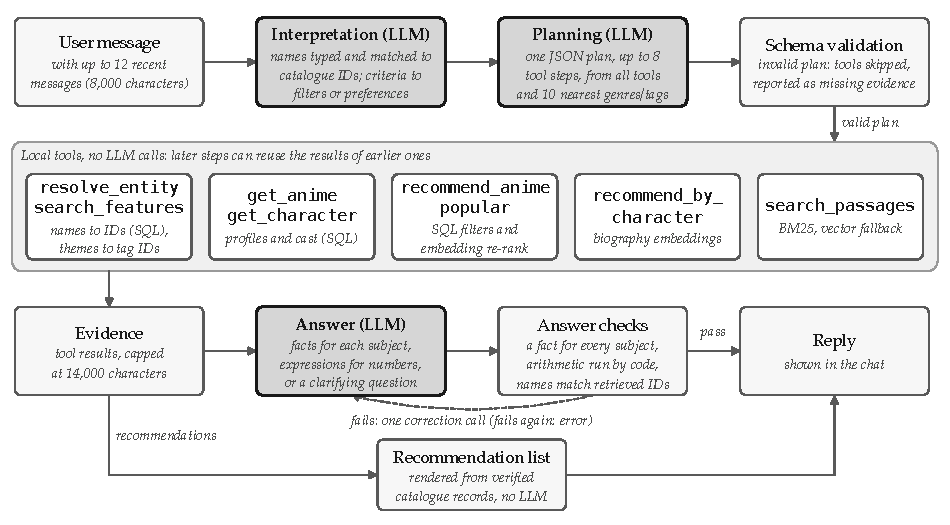
\includegraphics[width=\linewidth]{figures/agent_flow.pdf}
    \caption{Query flow inside the agent: one planning call (dark), local tool execution without LLM calls, one answer call (dark). The dashed arrow is the optional correction call.}
    \label{fig:agent}
\end{figure}

\textbf{Agent.} Each request passes through three stages. \emph{Planning:} the agent keeps up to 12 recent messages (at most 8,000 characters) but discards them when the message is a self-contained recommendation request, so that earlier constraints do not leak into a new search. Titles and characters named in the message are looked up in the dictionaries and their profiles are preloaded as evidence. The message is then embedded to retrieve the four most relevant tool descriptions and the ten closest genre and tag candidates. With this context, the \emph{planner} LLM produces a single JSON plan stating whether earlier context applies, the goal of the response, an optional clarification request, and up to eight tool steps with their arguments. \emph{Execution:} the plan is validated against a schema and executed locally without further LLM calls; if validation fails, no tool runs and the failure is passed to the answer stage as missing evidence. The tools resolve names to catalogue identifiers (\texttt{resolve\_entity}), load anime and character profiles from SQL (\texttt{get\_anime}, \texttt{get\_character}), rank SQL candidates, optionally re-ranked by embedding similarity to a stated preference (\texttt{recommend\_anime}, \texttt{popular}), find anime with similar main characters through biography embeddings (\texttt{recommend\_by\_character}), and retrieve descriptive passages with BM25 full-text search and a vector-search fallback (\texttt{search\_passages}). A step may reference the output of an earlier step. \emph{Answering:} the evidence, capped at 14,000 characters, is passed to the \emph{answer} LLM, which writes the reply from this evidence alone, reports missing information or asks for clarification. A final check compares the anime and characters named in the reply with the retrieved identities; on a mismatch, one correction call is made, and if the mismatch persists an error is returned instead of the answer. Locally, both LLM roles use \texttt{llama3.2:3b}~\cite{llama32} through Ollama, with temperature 0.2, a context window of 8,192 tokens and at most 700 output tokens.

\textbf{Design choices.} Planning all steps in advance bounds each answer to two LLM calls (three with a correction), whereas an interleaved reasoning-and-acting loop~\cite{yao2023react} requires one call per tool step; decoupling planning from tool observations follows ReWOO~\cite{xu2023rewoo} and keeps latency and cost predictable. Factual questions, such as the number of episodes, have a single correct answer, which an exact SQL look-up returns reliably and a nearest-neighbour search may miss; semantic search is therefore reserved for vague requests. Because the tools perform the retrieval, a small 3B model suffices for planning and phrasing, which keeps the system inexpensive and able to run on a laptop. Each request logs its plan, tool calls and stage timings, which supports debugging and transparency.

\begin{figure}[H]
    \centering
    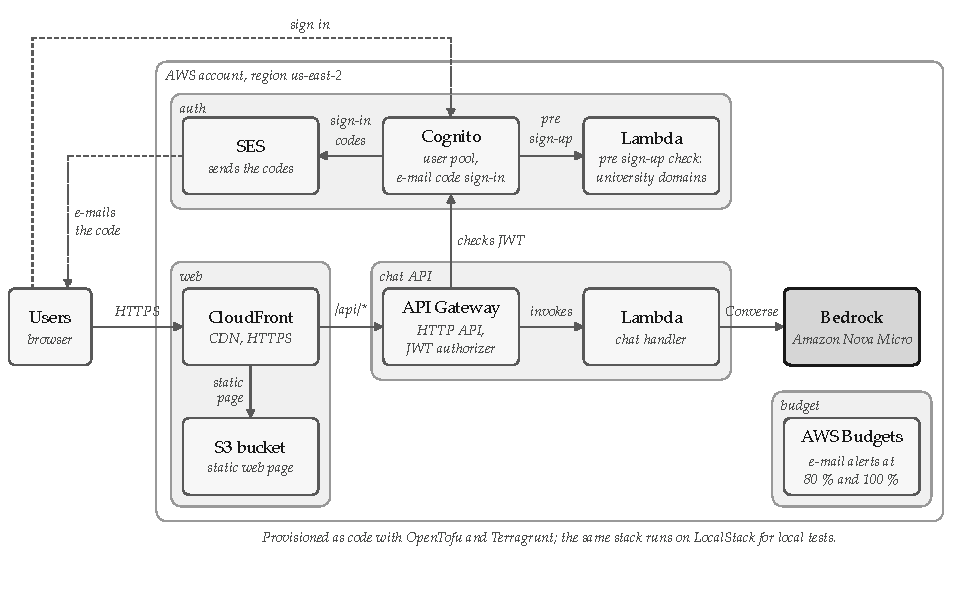
\includegraphics[width=\linewidth]{figures/aws_architecture.pdf}
    \caption{Deployment on AWS. Dashed arrows: the user's sign-in. Shaded regions are infrastructure units deployed separately.}
    \label{fig:aws}
\end{figure}

\textbf{Deployment.} Users open a static page that CloudFront serves from a private S3 bucket. Sign-in is passwordless: Amazon Cognito sends a one-time code through Amazon SES, and a pre-sign-up Lambda function rejects addresses outside \texttt{uu.se} and \texttt{student.uu.se}. CloudFront forwards requests under \texttt{/api/*} to an API Gateway HTTP API, whose JWT authorizer validates the Cognito token before a Lambda function processes the message and calls Gemma~3~4B~\cite{gemma3} on Amazon Bedrock through its OpenAI-compatible Chat Completions endpoint (\texttt{bedrock-mantle}). The Lambda signs these requests with its own IAM role, so no API key is stored; a configuration switch selects the Bedrock Converse API instead, which LocalStack uses. \TODO{PR \#6 is not merged yet; describe how the agent of PR \#5 runs behind the chat Lambda and which model the final demo uses} An AWS budget sends e-mail alerts when actual spend exceeds 80\% or forecast spend exceeds 100\% of the monthly limit. The infrastructure is defined as code with OpenTofu modules and Terragrunt environments and is tested automatically in GitHub Actions. LocalStack emulates the same stack locally at no cost, replacing Bedrock with the small \texttt{qwen2.5:0.5b} model, which tests the request path but not answer quality. Serverless components suit the low and irregular load of a demonstration: they incur no cost when idle and require no server maintenance. Restricting sign-in to university addresses also limits the audience, which matters for privacy and content (Section~\ref{sec:societal}).


\section{Results}
\instructions{In this section, present the outcomes of your experiments or evaluations. Provide both quantitative results (e.g., accuracy, precision, recall, BLEU, latency) and qualitative analyses (e.g., case studies, user feedback, example outputs). Where possible, compare the performance of your system against baseline methods or alternative approaches. Discuss the strengths of your application as well as its limitations, including cases where it may fail or underperform. Use tables, graphs, or figures to support clarity and emphasize key findings.}

\TODO{waiting for the evaluation. Status on 17 October: Aufa's evaluator for factual questions is running (not pushed yet); the recommendation evaluation is still to be decided; Aufa measures 20--30\,s per answer with llama3.2:3b on a desktop GPU, Tommi is measuring on a 64\,GB Apple-silicon laptop. Planned content:
(1) test set: how many questions, of which types;
(2) factual questions scored against the catalogue (SQL ground truth);
(3) recommendation questions (method to be decided);
(4) latency per stage (planning, tools, answer) from the request timings, with the hardware stated;
(5) a baseline, e.g. the same model without tools;
(6) two or three example conversations and failure cases.
All numbers must come from the setup used in the demo (local llama3.2:3b or Gemma 3 4B on Bedrock).}


\section{Societal Impact}
\label{sec:societal}
\instructions{Here, reflect on the broader implications of your LLM application for society. Discuss potential benefits such as improved accessibility, efficiency, education, or democratization of knowledge. At the same time, critically examine possible risks, including issues of bias, fairness, privacy, misuse, or environmental impact. Consider ethical challenges and describe mitigation strategies, such as transparency, safety mechanisms, or human oversight. This section should demonstrate awareness of the responsibility associated with deploying LLM-based systems in real-world contexts.}

\textbf{Benefits.} The assistant makes a large catalogue searchable in natural language, including by mood or by a liked character, without requiring knowledge of genre or tag names. Grounding answers in catalogue records and reporting missing information are intended to reduce fabricated titles and facts \TODO{support with Results}. Because a 3B model suffices, the agent can also run entirely on a user's own computer, so that no conversation leaves the device.

\textbf{Privacy.} The deployed system processes personal data of students and staff and is therefore subject to the GDPR~\cite{gdpr}. E-mail addresses are stored for sign-in; API and CDN logs record IP addresses and user agents; the Cognito user identifier is logged when a model call fails; chat messages are sent to Bedrock through the stateless Chat Completions API and are not stored by us. The current deployment runs in the AWS region \texttt{us-east-2}, outside the EU. Use beyond the course demonstration, which the teaching assistants approved, would require moving the stack to an EU region (\texttt{eu-north-1}) where the chosen model is offered, a data processing agreement with the university as controller, a record of processing activities, log retention limits, and disabled model invocation logging. \TODO{check with German which of these are done by the demo}

\textbf{Data provenance and copyright.} As discussed in Section~2, the CC0 label does not reflect the rights in the content: the AniList terms restrict mass collection and commercial use~\cite{anilist_terms}, many synopses are copyrighted third-party texts, and recommendations are contributed by AniList users. Our use is limited to a non-commercial educational project; a public or commercial service would require permission from AniList and licensed or original synopses. \TODO{check whether the raw dataset is excluded from the repository}

\textbf{Bias and fairness.} The ranking favours popular titles. Recommendations based on a reference title are ordered by AniList users' recommendation votes, then by shared genres and tags, then by popularity; requests without a reference title, the \texttt{popular} tool and ambiguous character names fall back to popularity order. This may reinforce a popularity feedback loop and reduce the visibility of lesser-known works. Scores and popularity reflect the AniList community rather than all viewers, and the English-only text limits access for speakers of other languages.

\textbf{Misuse and content safety.} Titles flagged as adult content are retained, because access is restricted to university students and staff, whom we assume to be adults; a public deployment should filter them by default. User messages reach the planner LLM, so prompt injection cannot be excluded. Its effect is limited because plans must pass schema validation, all tools are read-only, and answers are checked against the retrieved identities.

\textbf{Environmental and economic cost.} Small models (a local 3B model and Gemma 3 4B in the cloud) and at most three LLM calls per answer keep energy use and cost low. Bedrock charges per token, so the budget alerts guard against unexpected spending, and development runs on LocalStack rather than on the paid cloud.


\hfill \break
\textit{\textbf{Use of generative AI}}

\instructions{Write a few sentences if you have or have not used any generative AI, and if so how.}

\TODO{write the declaration}


\hfill \break
\textit{\textbf{Note}}

\instructions{Report should be max. 4-6 pages long.}


\begin{thebibliography}{10}

	%\bibitem{Item} Add here.

	\bibitem{anilist_kaggle} Caleb. \emph{Anilist Anime Dataset}, version 100. Kaggle, 2026. \url{https://www.kaggle.com/datasets/calebmwelsh/anilist-anime-dataset}

	\bibitem{anilist_terms} AniList. \emph{AniList API Terms of Use}. \url{https://docs.anilist.co/guide/terms-of-use}, accessed 17 October 2026.

	\bibitem{ji2023hallucination} Z.~Ji et al. Survey of hallucination in natural language generation. \emph{ACM Computing Surveys}, 55(12):1--38, 2023.

	\bibitem{lewis2020rag} P.~Lewis et al. Retrieval-augmented generation for knowledge-intensive NLP tasks. In \emph{Advances in Neural Information Processing Systems 33 (NeurIPS 2020)}, 2020.

	\bibitem{reimers2019sbert} N.~Reimers and I.~Gurevych. Sentence-BERT: sentence embeddings using Siamese BERT-networks. In \emph{Proceedings of EMNLP-IJCNLP 2019}, 2019.

	\bibitem{llama32} Meta. \emph{Llama 3.2 model card}. 2024. \url{https://github.com/meta-llama/llama-models/blob/main/models/llama3_2/MODEL_CARD.md}

	\bibitem{gemma3} Gemma Team. Gemma 3 technical report. \emph{arXiv:2503.19786}, 2025.

	\bibitem{yao2023react} S.~Yao et al. ReAct: synergizing reasoning and acting in language models. In \emph{International Conference on Learning Representations (ICLR)}, 2023.

	\bibitem{xu2023rewoo} B.~Xu et al. ReWOO: decoupling reasoning from observations for efficient augmented language models. \emph{arXiv:2305.18323}, 2023.

	\bibitem{gdpr} Regulation (EU) 2016/679 of the European Parliament and of the Council of 27 April 2016 (General Data Protection Regulation). \emph{Official Journal of the European Union}, L 119, 4 May 2016, pp.~1--88.

\end{thebibliography}



%	\pagebreak
%
%	\appendix
%	\section{Code}
%	\label{app:code}
%
%	\inputminted[frame=lines,framesep=2mm,linenos]{python}{your_code.py}
%
\end{document}
